\documentclass{article}

% \usepackage[ansinew]{inputenc} %Bærbar ÆØÅ?

\usepackage{minted}
\usepackage{graphicx} % Allows figures
% \usepackage{tabularx}
\usepackage{amsmath} %math
%Section style
\usepackage{etoolbox} %for configuration of sloppy
\usepackage{xcolor}

\definecolor{secnum}{RGB}{102,102,102}

\makeatletter
    \def\@seccntformat#1{\llap{\color{secnum}\csname the#1\endcsname\hskip 16pt}}
\makeatother
%end section style

{\sloppy}{\hbadness 10000\relax}{}{} %adds hbadness to sloppy
\setlength{\paperheight}{297mm} %Sets the page to an A4
\setlength{\paperwidth}{210mm}        %Sets the page to an A4

\begin{document}

\begin{titlepage}
\begin{center}
\textsc{Introduction to Graphics}\\[0.5cm]
\textsc{Assignment 5: Bezier Curves}\\[0.5cm]
\vspace{2 cm}
\begin{tabular}{ll}
Student: & Kasper Passov\\
\end{tabular}
\end{center}
\vspace{5 cm}
\newpage
\end{titlepage}

\section{Bezier curves}
A Bezier curve is created by two matrices, a \emph{Basic matrix} and a \emph{Geometry matrix}. The 
\emph{Geometry matrix} contains 4 vectors called \emph{Control Points}, descriping the placement 
and shape of the matrix. The first and fourth vector descripes the start and endpoint of the
curve, where the secound and third are points along the curve, not necessarily on the curve.
The \emph{Basic matrix} is used to transform the curve into a Hermit curve.

\section{Implementation}
I implemteted all types of line calculations in the mouseBeizer framework.

\subsection{Sampling}
The sampling was implemented in the given framework, so no work was done on it.
\begin{minted}{cpp}
Point drawBezierSample(Point A, Point B, Point C, Point D, double t) 
{ 
    Point P;
    P.x = pow((1 - t), 3) * A.x + 3 * t * pow((1 -t), 2) * B.x + 
             3 * (1-t) * pow(t, 2)* C.x + pow (t, 3)* D.x;
    P.y = pow((1 - t), 3) * A.y + 3 * t * pow((1 -t), 2) * B.y + 
             3 * (1-t) * pow(t, 2)* C.y + pow (t, 3)* D.y;
	P.z = 0;
    return P;
\end{minted}
The sampling is a naive implementation of the equation for a parametric curve
\begin{equation*}
    f(t) = at^3 + bt^2 + ct + d
\end{equation*}
Where the linesegments are calculated by the for loop in the main function
\begin{minted}{cpp}
for(double t = 0.0;t <= 1.0; t += 1.0/n) {
    Point P = drawBezierSample(abc[0], abc[1], abc[2], abc[3],  t);
    drawLine(POld, P);
    POld = P;
\end{minted}
This loop handles the increments of $t$, so we have calculated points equaly constributed along the curve,
with $1/n$ between each point.

\subsection{Forward Differencing}
Using forward differencing we can reduce the cost of evaluation to only 3 additions per curvepoint.
By using \delta\ we can remove the t variable, replacing it with the variable that defines the interval
of the point calculations. This means we can replace the variable $t$ with the constant \delta\ making the
calculations a lot simpler.\\
The matrix is defined in the function
\begin{minted}{cpp}
void forwardDiffInit(Point A0, Point B0, Point C0, Point D0, double del, Point deltas[]){
    Point fda = (A0 * -1.0) + (B0 *  3.0) + (C0 * -3.0) + D0;
    Point fdb = (A0 *  3.0) + (B0 * -6.0) + (C0 *  3.0);
    Point fdc = (A0 * -3.0) + (B0 *  3.0);
    Point fdd =  A0;

    deltas[0] = fdd;
    deltas[1] = fda *     pow(del, 3.0) + fdb * pow(del, 2.0) + fdc * del;
    deltas[2] = fda * 6.0 * pow(del, 3.0) + fdb * 2.0 * pow(del, 2.0);
    deltas[3] = fda * 6.0 * pow(del, 3.0);
\end{minted}
With this we can calculates the points using the itteration defined in the following function 
\begin{minted}{cpp}
point drawbezierforwarddiff(point deltas[]) {
    point p;
    p = deltas[0];

    deltas[0] = deltas[0] + deltas[1];
    deltas[1] = deltas[1] + deltas[2];
    deltas[2] = deltas[2] + deltas[3];
	return p;
\end{minted}
The itterations of t is much the same, but with the addition of the initiation of the delta vector.

\subsection{Subdivision}
In my implementation of subdivision i ran into one large problem i am yet to solve. After calculating a point
on the middle of the curve recursivly, i need to sort these points, so the points are connected in the correct order.
This is a problem as the algorithm does not calculate them in the correct order. This i tried to get around by creating
a recursive function, that creates a tree structure forcing the leftmost calculated point on the curve to be calculated
first.
\begin{minted}{cpp}
void drawBezierSubdivision(Point G1, Point G2, Point G3, Point G4, double n) {
    ...
    drawBezierSubdivision(Left[0], Left[1], Left[2], Left[3], floor(n/2)); 
    P = Left[0];
    drawLine(POld, P);
    POld = P;
    drawBezierSubdivision(Right[0], Right[1], Right[2], Right[3], ceil(n/2)-1); 
\end{minted}
The values of the Left and Right vector is calculated above the recursive call. 
I ensure the right amount of points are calculated by checking ageinst a n value
that each recursive call get half of. If a call gets a value of 0, the point
is not drawn.

\section{Testing}
I created some curves with each of the 3 methods. Further testing can be done making and running the zipped file.
\subsection{Sampling}
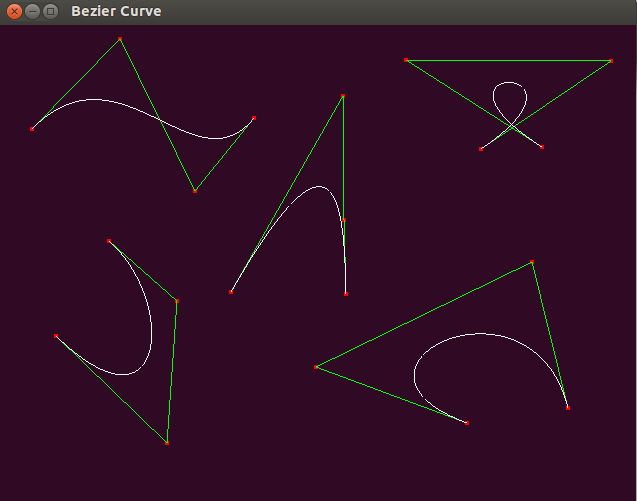
\includegraphics[scale=0.4]{SamplePenis.png}\\
\subsection{Forwarding}
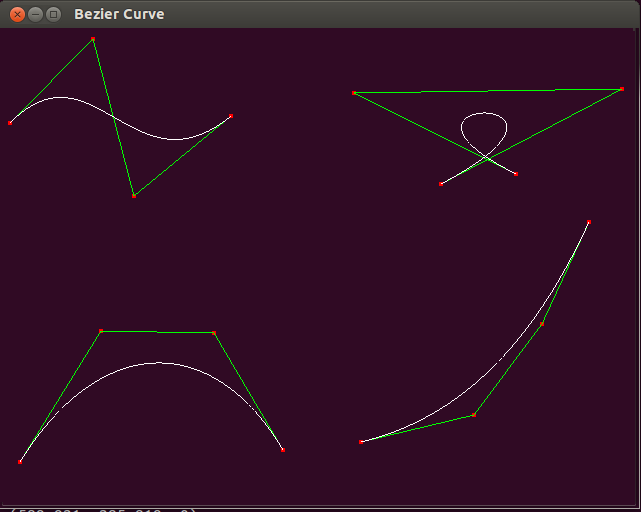
\includegraphics[scale=0.4]{ForwardPenis.png}\\
\subsection{Subdivision}
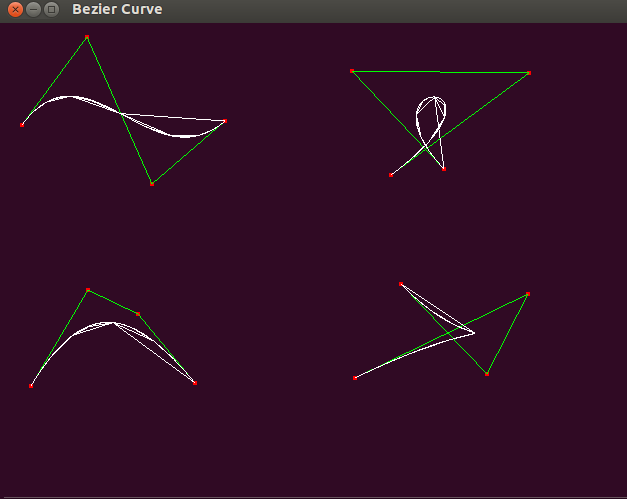
\includegraphics[scale=0.4]{subpenis.png}\\


\end{document}

